%% ----------------------------------------------------------------
%% Thesis.tex -- MAIN FILE (the one that you compile with LaTeX)
%% ---------------------------------------------------------------- 

% Set up the document
\documentclass[a4paper, 11pt, oneside]{Thesis}  % Use the "Thesis" style, based on the ECS Thesis style by Steve Gunn
\graphicspath{{./Figures/}}  % Location of the graphics files (set up for graphics to be in PDF format)

% Include any extra LaTeX packages required
\usepackage[ ]{biblatex}
\addbibresource{library.bib}
% \usepackage[square, numbers, comma, sort&compress]{natbib}  % Use the "Natbib" style for the references in the Bibliography
\usepackage{verbatim}  % Needed for the "comment" environment to make LaTeX comments
\usepackage{vector}  % Allows "\bvec{}" and "\buvec{}" for "blackboard" style bold vectors in maths
\hypersetup{urlcolor=blue, colorlinks=true}  % Colours hyperlinks in blue, but this can be distracting if there are many links.
\usepackage{multirow}
\usepackage{makecell}
\usepackage[capitalise]{cleveref}

\begin{document}
%% ----- Cover ----------------------------------------------------
  \frontmatter      % Begin Roman style (i, ii, iii, iv...) page numbering

  % Set up the Title Page
  \title {Autonomous Navigation Behaviors for an Aerial Robotics Software Framework}
  \authors {
    \texorpdfstring{
      Guillermo Echegoyen Blanco
    }
    {Guillermo Echegoyen Blanco}
  }
  \addresses {
    \groupname\\\deptname\\\univname
  }  % Do not change this here, instead these must be set in the "Thesis.cls" file, please look through it instead
  \date {\today}
  \subject {}
  \keywords {}

  \maketitle
%% ----------------------------------------------------------------
%% ----- Page Setup -----------------------------------------------
  \setstretch{1.3}  % It is better to have smaller font and larger line spacing than the other way round

  % Define the page headers using the FancyHdr package and set up for one-sided printing
  \fancyhead{}  % Clears all page headers and footers
  \rhead{\thepage}  % Sets the right side header to show the page number
  \lhead{}  % Clears the left side page header

  \pagestyle{fancy}  % Finally, use the "fancy" page style to implement the FancyHdr headers
%% ----------------------------------------------------------------
%% ----- Declaration Page -----------------------------------------
  % Declaration Page required for the Thesis, your institution may give you a different text to place here
  \Declaration{

    \addtocontents{toc}{\vspace{1em}}  % Add a gap in the Contents, for aesthetics

    I, AUTHOR NAME, declare that this thesis titled, `THESIS TITLE' and the work presented in it are my own. I confirm that:

    \begin{itemize} 
      \item[\tiny{$\blacksquare$}] This work was done wholly or mainly while in candidature for a research degree at this University.
       
      \item[\tiny{$\blacksquare$}] Where any part of this thesis has previously been submitted for a degree or any other qualification at this University or any other institution, this has been clearly stated.
       
      \item[\tiny{$\blacksquare$}] Where I have consulted the published work of others, this is always clearly attributed.
       
      \item[\tiny{$\blacksquare$}] Where I have quoted from the work of others, the source is always given. With the exception of such quotations, this thesis is entirely my own work.
       
      \item[\tiny{$\blacksquare$}] I have acknowledged all main sources of help.
       
      \item[\tiny{$\blacksquare$}] Where the thesis is based on work done by myself jointly with others, I have made clear exactly what was done by others and what I have contributed myself.
      \\
    \end{itemize}
   
     
    Signed:\\
    \rule[1em]{25em}{0.5pt}  % This prints a line for the signature
     
    Date:\\
    \rule[1em]{25em}{0.5pt}  % This prints a line to write the date
  }
  \clearpage  % Declaration ended, now start a new page
%% ----------------------------------------------------------------
%% ----- Funny Quote ----------------------------------------------
  % The "Funny Quote Page"
  \pagestyle{empty}  % No headers or footers for the following pages

  \null\vfill
  % Now comes the "Funny Quote", written in italics
  \textit{``Write a funny quote here.''}

  \begin{flushright}
    If the quote is taken from someone, their name goes here
  \end{flushright}

  \vfill\vfill\vfill\vfill\vfill\vfill\null
  \clearpage  % Funny Quote page ended, start a new page
%% ----------------------------------------------------------------
%% ----- Abstract Page --------------------------------------------
  % The Abstract Page
  \addtotoc{Abstract}  % Add the "Abstract" page entry to the Contents
  \abstract{
    \addtocontents{toc}{\vspace{1em}}  % Add a gap in the Contents, for aesthetics

    The Thesis Abstract is written here (and usually kept to just this page). The page is kept centered vertically so can expand into the blank space above the title too\ldots
  }
  \clearpage  % Abstract ended, start a new page
%% ----------------------------------------------------------------
%% ----- Acknowledgements page ------------------------------------
  \setstretch{1.3}  % Reset the line-spacing to 1.3 for body text (if it has changed)
  % The Acknowledgements page, for thanking everyone
  \acknowledgements{
    \addtocontents{toc}{\vspace{1em}}  % Add a gap in the Contents, for aesthetics

    The acknowledgements and the people to thank go here, don't forget to include your project advisor\ldots
  }
  \clearpage  % End of the Acknowledgements
%% ----------------------------------------------------------------
%% ----------------------------------------------------------------
%% ----- Contents, List of Figures, List of Tables ----------------
  \pagestyle{fancy}  %The page style headers have been "empty" all this time, now use the "fancy" headers as defined before to bring them back
  
  \lhead{\emph{Contents}}  % Set the left side page header to "Contents"
  \tableofcontents  % Write out the Table of Contents
  
  \lhead{\emph{List of Figures}}  % Set the left side page header to "List if Figures"
  \listoffigures  % Write out the List of Figures

  \lhead{\emph{List of Tables}}  % Set the left side page header to "List of Tables"
  \listoftables  % Write out the List of Tables
  \setstretch{1.5}  % Set the line spacing to 1.5, this makes the following tables easier to read
  \clearpage  % Start a new page
%% ----------------------------------------------------------------
%% ----- Abbreviations, Physical Constants, Symbols ---------------
  \begin{comment}
  \lhead{\emph{Abbreviations}}  % Set the left side page header to "Abbreviations"
  \listofsymbols{ll}  % Include a list of Abbreviations (a table of two columns)
  {
    % \textbf{Acronym} & \textbf{W}hat (it) \textbf{S}tands \textbf{F}or \\
    % \textbf{LAH} & \textbf{L}ist \textbf{A}bbreviations \textbf{H}ere \\
  }
  \clearpage  % Start a new page

  \lhead{\emph{Physical Constants}}  % Set the left side page header to "Physical Constants"
  \listofconstants{lrcl}  % Include a list of Physical Constants (a four column table)
  {
    % Constant Name & Symbol & = & Constant Value (with units) \\
    % Speed of Light & $c$ & $=$ & $2.997\ 924\ 58\times10^{8}\ \mbox{ms}^{-\mbox{s}}$ (exact)\\
  }
  \clearpage  %Start a new page

  \lhead{\emph{Symbols}}  % Set the left side page header to "Symbols"
  \listofnomenclature{lll}  % Include a list of Symbols (a three column table)
  {
    % symbol & name & unit \\
    % $a$ & distance & m \\
    % & & \\ % Gap to separate the Roman symbols from the Greek
    % $\omega$ & angular frequency & rads$^{-1}$ \\
  }
  \end{comment}
%% ----------------------------------------------------------------
% End of the pre-able, contents and lists of things
%% ----- Dedication Page ------------------------------------------
  % Begin the Dedication page
  \setstretch{1.3}  % Return the line spacing back to 1.3

  \pagestyle{empty}  % Page style needs to be empty for this page
  \dedicatory{For/Dedicated to/To my\ldots}

  \addtocontents{toc}{\vspace{2em}}  % Add a gap in the Contents, for aesthetics
%% ----------------------------------------------------------------
%% ----- Main Document --------------------------------------------
  \mainmatter   % Begin normal, numeric (1,2,3...) page numbering
  \pagestyle{fancy}  % Return the page headers back to the "fancy" style

  \renewcommand{\chaptermark}[1]{\markboth{#1}{}} % Make the chapter mark without the "Chapter X" stuff
  \lhead{\emph{\leftmark}}  % Set the left side page header accordingly

  \chapter{Introduction}

  In the following work an integration of a navigation system onto the Aerostack platform is presented.

  \section{Context}

    Aerostack is a framework for aerial robots, aimed at giving flight autonomy to some extent. It features a modular approach for the construction of behaviors that can be used to develop complex flights and automatic handling for certain situations such battery level or hardware conditions. It is the frame for the following work, which adds more autonomy through the integration of a octomap-based navigation system and a global planner. This provides a novel localization technique for the framework.

  \section{Motivation}

    So far, there exists only one simple geometry planner and an Aruco-based localization technique. In indoor environments, this system compels the need for environment preparation, the Arucos must be placed beforehand in well known localizations that must be hardcoded in the robot map. In this sense, there exists a need for a more robust, preparation-free localization system and accompanying planner. This work provides such an improvement with the introduction of a octomap-based navigation system and a global planner.

  \section{General Objective}

    This work aims at adding a novel navigation system to the Aerostack framework.


  \section{Specific Objectives}

    This section enumerates a comprehensive list of objectives.

    \begin{enumerate}
      \item Enrich the current navigation and localization systems.
      \item Test and validate the new navigation and localization systems through simulated environments.
    \end{enumerate}

    To achieve the first objective, the following additions to the framework are proposed:

    \begin{itemize}
      \item Add a robust planner based on a new navigation technique.
      \item Add a robust navigation technique through the use of octomaps.
      \item Add a robust localization technique based on octomaps.
      \item Add octomaps construction support through lidar.
    \end{itemize}

  \section{Overview}

    \textbf{[ToDo := Review when everything is finished]}

    This dissertation is organized as follows: ...

 % Introduction

  \chapter{Problem Description}

  In the present chapter the problem is presented, along with an introduction to the previous work. It is structured as follows: Section \ref{ch_2:sect:1} presents the context of the problem and the requirements a replacement should have. Section \ref{ch_2:sect:2} describes deeply the improvements presented and the decisions taken to end in Section \ref{ch_2:sect:3} with the description of the previous system.

  \section{Requirements} \label{ch_2:sect:1}

    As of the second version of Aerostack, the only localization technique available is based on the recognition of a special type of marker called Aruco, first used for augmented reality applications. It is a fast and reliable technique to estimate the pose of the camera capturing the image. Altough this system works fine for many applications, it imposes the need of preparing the environment, placing this markers in a very precise way and annotating it's exact position before the experiments. While this might not be a problem in an augmented reality like scenario, when it comes to live localization in unknown environment it becomes useless. Hence, a new system for localization is required.

    Along with the aforementioned localization technique comes the navigator which coordinates with a 2D geometric planner to accomplish the mission at hand. As the localization technique is to be changed, leading to a new way to perceive the environment, a new navigator and planner will be necessary. 

  \section{Details of the New Features} \label{ch_2:sect:2}

    A lidar is going to be used as the main source for localization. The module in charge of this part is already present in the Aerostack framework, but it is not being used. Based on lidar input an octomap is built. This octomap is then used by the navigator, along with the planner instructions to build a motion plan to execute.

    The lidar + octomap functionality is provided by a module called hector\_slam, developed at the Darmstadt University \cite{hector_slam}. Taking the lidar's cloud of points it is able to reconstruct an octomap and then localize inside it (SLAM). The output of this module can be used to create a plan avoiding obstacles to reach a target point.

    [ ToDo := Review, NavStack \& Global Planner ]

  \section{Previous Work} \label{ch_2:sect:3}

    By now, there is a process responsible for doing recognition of Aruco markers, it is connected to the robot camera and fetches data every $n$ milliseconds, where $n$ is a user defined constant. When an aruco is recognized, the pose of the robot can be estimated. Knowing the exact position of the marker enables the process to estimate the absolute position of the robot, leading to a high precision coordinates localization. While this approach has many advantages, it fails when the environment is not prepared beforehand.

    To create a plan, a target position and the used Aruco markers are specified, then the motion planner creates a 2D plan to follow, using the Arucos to localize in the process.

    \begin{comment}
      \begin{itemize}
      \end{itemize}
    \end{comment}

 

  \chapter{State of the Art}

  This chapter will review the classic methods used for localization and mapping, which is the core for any navigation technique, it starts describing the problems that arise both in localization and mapping. Continue with some of the most prolific solutions found to these problems to finish exposing the techniques and algorithms used by the Aerostack framework.

  Localization is referred to all the techniques used to find the position in coordinates of an agent or object inside the world, relative to a reference frame. As far as it's absolute coordinates are known, anything can be used as reference frame, it is used as the coordinates system's centre. In an outdoors environment, the Earth could be the reference frame and the robot's coordinates can be acquired with satellite systems, giving an absolute point inside the three dimensional space. It is desirable for these coordinates to be in a format that a computer can handle efficiently, tipically as two or three floating point numbers (although integer numbers are used sometimes too), depending on the number of dimensions used to represent the space. To save computational effort, the z axis (height) could be unused in a wheeled robot.

  Moving a robot avoiding possible obstacles through the space is tricky in itself, obstacles must be detected and handled correctly, moving objects can appear in the way, and so on. This alone does not provide any intelligence nor it helps planning, to aid in planning and moving smartly in the space, a map can be constructed while the localization is happening. The term mapping covers all the algorithms used to construct a map combining the data acquired from the many input sources a robot can have. Mapping opens the door for smart planning, along with many more advantages. A classic example is finding cycles in planned paths.

  \clearpage

  \section{Localization}

    Localization techniques are divided into two groups: Outdoor and indoor techniques. The distinction comes from the fact that satellite systems signals cannot go through walls. This fact has led to a whole new set of technologies and techniques that are able to localize in environments without an absolute reference of the world.

    This section is organized as follows: First outdoor localization will be analyzed, with a brief review of it's core components, then various indoor localization techniques will be exposed, focusing on lidar based techniques.

    \subsection{Outdoor localization} \label{ch_3:sect:localization:outdoor}

      By now, the most robust, reliable solution for outdoor localization is based on combining different sources of data. The mobile platform has drawn great attention over the past few years, pushing some of the largest companies in a shared effort to improve localization services while minimizing the impact over the battery's performance.

      Satellite systems localization in mobile applications have certain drawbacks: The most obvious one is that acquiring and processing the signal wastes power, but also that in the case of civilian systems (such as GPS) the localization has a precision of 10 meters for security reasons. Figure \ref{ch_3:fig:trilateration} shows the localization dissambiguation through the trilateration technique with three satellite.

      To aid both problems two new localization techniques were implemented:
      \begin{enumerate}
        \item GSM Localization. As every GSM antenna has a well known location stored in a database, one can localize trilaterating the near GSM antennas. Obviosly, this method is subject to GSM signal coverage.
        \item WiFi Localization. This powerful method can serve both as an indoor and outdoor localization technique (see sect. \ref{ch_3:sect:localization:indoor}). When a smarphone detects a WiFi hotspot, it sends it's BSSID along with the GPS coordinates if available to a centralized server. As this database grows the localization precision improves and every user can take advantage from it. This is scpecially useful in urban areas where stallite signal is poor or intermitent and improves as more and more users log information.
      \end{enumerate}

      The best localization services can be provided with the conjunction of these three main techniques, which can be easily merged with an \textit{Extended Kalman Filter}.

      \begin{figure}
        \centering
        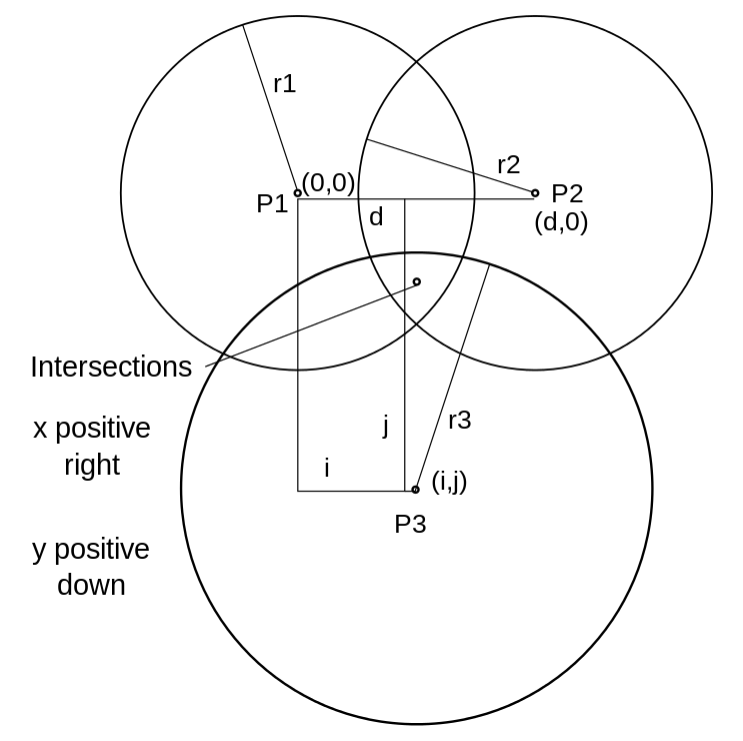
\includegraphics[width=0.6\textwidth]{./Figures/trilateration.png}
        \caption{The area enclosed by the three intersections ca be used to localize univocally. The three simple intersections formed by pairs of circumferences are always outside of the Earth. As more satellites are included, precision increases. Taken from \cite{wikipedia_trilateration_web}.}
        \label{ch_3:fig:trilateration}
      \end{figure}

      Although these techniques are widely used they are limited to mobile platforms, which are restricted both in sensorization and in processing capabilities. For robotic applications more sophisticated sensors are used, this includes depth cameras and lidars for the most part. Again, all the sensors output is merged to get the best estimates.

      In robotics, it is usual that the localization we are interested in is relative instead of absolute. This is done to aid in locating near objects in the space relative to the robot but also to construct a map, the process of localization and mapping simultaneously is called \textit{SLAM - Simultaneous Localization And Mapping} (see sect. \ref{ch_3:sect:localization:slam}).

    \subsection{Indoor localization} \label{ch_3:sect:localization:indoor}

      To localize in indoor environments many strategies can be followed, the general trend is to place different markers (active or passive) beforehand in well known locations. This markers are then recognized by the localizing device to know it's location. This \textit{recognizable markers} can be anything, a Bluetooth beacon, a WiFi hotspot, etc.

      Bluetooth beacons are specially crafted for this purpose as they can provide much more information. It has been extensively used in congresses and hotels to provide hosts with more information beyond localization, as services and timetables based on location. 

      In the case of WiFi hotspots localization is usually done by analyzing the signal strength and incoming angle. This method only works when the hotspots' location is known beforehand and is very prone to errors because the device must remain static in a certain angle.

      From the computer vision perspective, visual markers can be placed too and processed by the device localizing and again, this requires preparation beforehand. One example of this setup are the well known \cite{romeroramirez201838}.

      In many robotic applications like swarm robotics there is a necessity to track each member of the swarm in a closed, contained environment, for this purpose an OptiTrack system \cite{optitrack_web} can be used, it is a highly precise camera set that can track various markers (marked swarm members) and serve it's location through the network in real time. This setup is specially useful to monitor the swarm, enabling each member to access it's location.

    \subsection{SLAM} \label{ch_3:sect:localization:slam}

      SLAM is the process of mapping and, at the same time localizing inside that map. This is particularly useful in environments that are not prepared like the ones exposed previously, enabling the robot to work on an unknown place without getting lost nor entering cyclic paths. SLAM techniques are crucial in any robot with some degree of autonomy, it makes the navigation possible. 

      There are three main variants here, the ones based on Extended Kalman Filters, the probabilistic ones and the ones based on Graph Optimization.

    \subsubsection{Extended Kalman Filters SLAM} \label{ch_3:sect:localization:ekf}

      Extended Kalman Filters (EKF) SLAM is the earliest technique developed for SLAM. EKF is a general technique to find the best estimate for the measuring variable based on the mean and covariance. In this case the inputs are the odometry used to estimate the robot position, features of the environment that anchor the odometry measures and the robot motor system sensors (wheel decoders, etc) to estimate the change on the position. Then the objective is to find the best estimate for the current robot's position.

      \begin{figure}[!t]
        \centering
        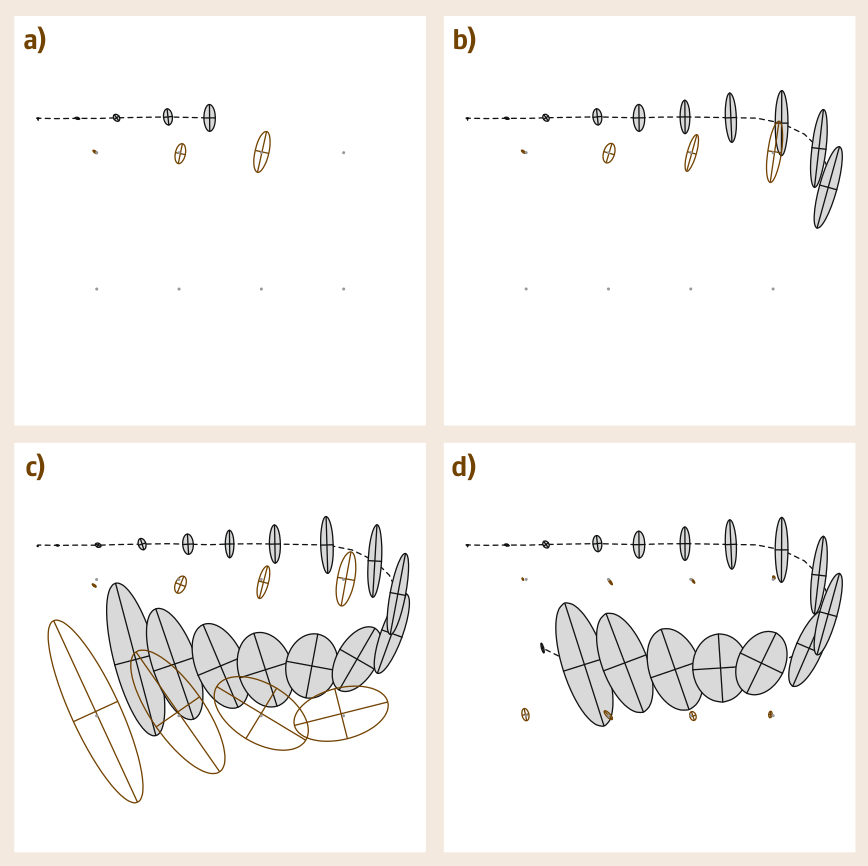
\includegraphics[width=0.8\textwidth]{./Figures/slam_ekf_model.png}
        \caption{EKF applied to the SLAM problem. Dotted line: robot's path. Shaded ellipses: position estimates. Small dots: Unkown location landmarks. White ellipses: Landmarks' position estimates. In (d) the robot senses the first landmark, anchoring the rest of the estimates, reducing uncertainty. Taken from \cite{inbookhandbook}}
        \label{ch_3:fig:ekf_slam}
      \end{figure}

      At the start of the process, the system's ($0$, $0$) coordinate is established where the robot is, this is the most confident measure about the robot position. As the robot navigates the environment, succesive measures are taken and paired with the known landmarks, when a previously seen landmark is witnessed again, the position estimate is corrected with the covariance matrix, and the error correction is propagated along the previous estimates. In this way a long as the robot is navigating an sensing the landmarks, the position estimate improves. Figure \ref{ch_3:fig:ekf_slam} shows the full process, in (a) the process is started, there is a lot of uncertainty, as process continues (a-c) the uncertainty increases, until the first landmark is sensed again (c), reducing the uncertainty on the current position's estimate and the subsequent estimates.

      More formally, the EKF algorithm represents the robot estimate by a multivariate Gaussian (\ref{ch_3:eq:ekf_representation})
      
      \begin{equation} \label{ch_3:eq:ekf_representation}
        p(x_{t}, m | Z_{t}, U_{t}) = N(\mu_{t}, \Sigma_{t})
      \end{equation}

      Where $\mu_{t}$ contains the robot's best estimate of its current location $x_{t}$ and the locations of all the landmarks, its size is $3 + 2N$, 3 points for the robot location and 2 for each of the $N$ landmarks. The matrix $\Sigma_{t}$ is the covariance of the expected error in the guess $\mu_{t}$ assessed by the robot, a square, dense matrix of $(3 + 2N) \times (3 + 2N)$.

      Although this technique works well on small maps, it renders unusable for large maps, this happens because the covariance matrix $\Sigma_{t}$ used to correlate the position estimates grows cuadratically with the measures, making the memory footprint wildly large and the overall processing time very high. Some researchers have proposed an improvement over the EKF SLAM algorithm through submap decomposition \cite{Guivant2001, Leonard2000}.

    \subsubsection{Particle Filters}

      Particle Filters are a probabilistic approach to position estimation, usually called Fast SLAM \cite{Montemerlo2002}. It uses various \textit{particles} that represent the posterior probability of the true distribution of maps and possible paths. To do so it stands over a method called Rao-Blackwellization, that aids in dimensioning the number of particles needed to represent the map. Also, as conditional indepence is assumed between the observed landmarks, every landmark can be represented as $N$ small Gaussians, which is linear, instead of exponential on the number of landmarks.

      At any point a set of $K$ particles is retained, where each particle has the form exposed in equation \ref{ch_3:eq:particle_form}.

      \begin{equation} \label{ch_3:eq:particle_form}
        X_{t}^{[k]}, \mu_{t,1}^{[k]}, \cdots, \mu_{t,N}^{[k]}, \Sigma_{t,1}^{[k]}, \cdots, \Sigma_{t,N}^{[k]}
      \end{equation}

      Where $k$ is the index of the path sample and $n$ the number of the landmark. This implies that every particle contains a sample path $X_{t}^{[k]}$ and a set of $N$ Gaussians $\approx (\mu_{t,n}^{[k]}, \Sigma_{t,n}^{[k]})$, one for each landmark.

      When a new odometry measure is received, it is combined with the previous knowledge through probabilistic sampling. A new location is generated for each particle, following a distribution based on the robot motion model and the previous measure of that particle ($x_{t-1}^{[k]}$). More specifically:

      \begin{equation} \label{ch_3:eq:particle_update}
        x_{t}^{[k]} \approach p(x_{t} | x_{t-1}^{[k]}, u_{t})
      \end{equation}

      Then, when a new measure $z_{t}$ is received, each particle's importance is weighted, assigning how important is that particle to that measure, this is the probability of that measure based on the particle's knowledge, defined in equaton \ref{ch_3:eq:particle_importance}. Let $n$ be the observed landmark's index:

      \begin{equation} \label{ch_3:eq:particle_importance}
        w_{t}^{[k]} = N(z_{t} | x_{t}^{[k]}, \mu_{t,n}^{[k]}, \Sigma_{t,n}^{[k]})
      \end{equation}

      After equation \ref{ch_3:eq:particle_importance} is applied for each particle, all the weights are normalized to sum up to 1, then a set new particles is drawn with replacement, where the probability of being picked is each particle weigth. Intuitively, this means that only the particles that fit the most with the current measures survive for next rounds. The final step of FastSLAM updates the mean $\mu_{t}^{[k]}$ and covariance $\Sigma_{t,n}^{[k]}$ based on the new measure $z_{t}$, which is similar to the EKF updates, but with much smaller filters.

      Although this method is easy to implement, fast enough for real time applications with not very high demanding software and yields good results on small to medium maps, it suffers from the fact that lots of particles are needed to represent big maps, specially with multiple nested loops. Therefore, many improvements have been proposed, \cite{Grisetti2007} for example uses ocucupancy grids instead of Gaussians.

    \subsubsection{Graph Optimization SLAM}

      The Graph Optimization SLAM techniques try to optimize a graphical model representing the landmarks and robot locations. In this representation, each location is viewed as a node in the graph, and the edge (called soft constraint) between two consecutive nodes is the captured odometry. The key intuition behind these methods is that at the end, the graph is sparse, because, each node will have just a few connections to other nodes. Also, at worst, the number of entries in the graph is linear in the time elapsed and in the number of nodes.

      This is the most widely used approach because sparse linear optimization is in a very advanced stage, allowing for scalable, yet efficient implementations of the algorithm.

    \subsubsection{Lidar SLAM}

      Lidar is a well established laser range sensor that can be used for depth estimation. By doing fast sweeps in 360 degrees it can compose a depth map which can be used for SLAM.

      Hector SLAM \cite{hector_slam} is a technique developed in the Darmstadt University. It uses a lidar sensor to do a fast SLAM by matching rays along sweeps.

      Along this work, the \textit{hector\_slam} ROS module will be integrated into the Aerostack framework, providing a robust SLAM technique ready to use for the drones equiped with lidar.

    \subsubsection{Visual SLAM}

      Using computer vision for SLAM have been a challange since it's conception, it raises the difficulty, specially for monocular cameras. Although many features can be extracted from images, it is not clear how to process nor store the data taking into account the full 6 degrees of freedom in a camera. All the parameters of the camera must be known beforehand, depth cameras include a lot of noise and monocular cameras do not have scale.

      In \cite{murTRO2015}, ORB-SLAM is proposed. Intuitively, it creates ORB features from a visual input and stores it in a sparse matrix, then a matching process is launched to localize every feature, improving the localization along the way. It can work on Monocular (no scale), Stereo and Depth Cameras, giving extraordinary results.

  This chapter reviewed the main adversities inherent to the SLAM problem and shed some light over the current state of the art. In the rest of this document, we will focus solely on lidar SLAM as the drones used with Aerostack are bound to lidar sensors. 

  \begin{comment}
    \begin{itemize}
    \end{itemize}
  \end{comment}


  \chapter{Implemented Modules}

In this chapter, the technical goals of the project are introduced. Each developed module will be explained as well as it's requirements and specification details. For each module, the following points will be addressed:

\begin{itemize}
  \item The technical goals
  \item The problem to which the module provides a solution
  \item Some of it's properties (reusability, scalability \dots)
  \item Integration with the current version of Aerostack
\end{itemize}

\section{Technical Goals}

  In order for the Aerostack framework to localize with a different technique rather than visual markers a lidar sensor will be used. In this case, the \textit{Hokuyo Eye} range sensor will be used, which is the \textit{defacto} range sensor in this context. Also, the low level implentation provides a nice ros API that can be used to fetch data. To wrap all this functionallity we propose the implementation of a new high level behavior that coordinates all the framework with the lidar interface, providing a high level, standarized API for lidar-based localization.

  As of the current version of Aerostack, navigation is done with a 2D probabilistic roadmap planner, the input for the planner is a predefined map, done by hand in the Graphical User Interface that Aerostack provides. This is a static map and goes against the nature of the any dynamically acquired mapping signal. To tackle this problem several new navigation behaviors are proposed. These behaviors will abstract the planner used for each localization mode, providing a high level standarized API that can be used independently of the localization technique, replacing the old one.

\section{Specification}

  Each implemented module should follow the specification imposed by the Aerostack framework. In Aerostack there are different types of processes providing structure and added functionallity. When a new process is created it should be decided whether to implement it as a plain, simple ros node, a robot process or a behavior process. Their differences are as follows:

  \begin{itemize}
    \item ROS Node: This is the standard way of adding modules in a ROS oriented architecture. A ros node is simply a process programmed in any of the programming languages supported by ros (C, C++, Python \dots) that implements a task and is interfaced through the ros master server with named topics, services or both. A ros node can subscribe or publish topics and optionally, provide services, as many topics or services as it wants. These topics and services are nothing more than binded ports to the ROS master server, that works over TCP (normally) or UDP to distribute traffic. This is the implementation to follow when adding very low level modules, like platform drivers.
    \item Robot Process: A Robot Process is an abstraction provided by Aerostack, it serves mainly as a standarization layer, providing an interface for the rest of the architecture to be used. It provides three services to manage the process, one for stopping it, one for starting it and another one to check whether it is running or not, aditionally it emits an alive signal every second or an error signal when the thread crashes. It runs the inheritors' code inside a separate thread in order to monitor it. When adding a module that abstracts some low level APIs, like a visual marker processor, this is the class to inherit from.
    \item Behavior Process: This is the highest level of the hierarchy, inside the Aerostack framework there exists a process that coordinates all the behaviors, to do so, every behavior exposes an interface similar to the Robot Process and a configuration file that especifies the mid and low level processes the behavior depends upon (it's capabilities and incompabilities), amongst other parameters, in this sense, the behavior that provides localization based on visual markers depends on the visual marker processor to work. Formally, a behavior is just a high level process that monitors an algorithm: it runs the algorithm in a separate thread and emits the state and error signals, listening to \textit{start/stop} events and acting accordingly over the algorithm. When adding a high level functionallity, this is the class that should be inherited.
  \end{itemize}

  In a similar fashion to the visual marker localization behavior, the lidar localization behavior proposed will require three more processes: the slam process, an ekf that combines various signals and a localization technique selector, this is explained in detail in the corresponding behavior section (sect. \ref{ch_4:sect:behav_slam}).

  The navigation interface is slightly more complicated, it will be composed of various behaviors that provide different functionallity, abstracting away the logic needed to navigate at different levels. We propose three new behaviors and the inclusion of a new planner, efficiently designed to work with lidar signal. More details will be provided in the corresponding section \ref{ch_4:sect:nav_interface}

\section{Integration} \label{ch_4:sect:integration}

  To integrate each behavior, we will follow a bottom up procedure. This way, we will ensure that the processes the behavior depends on are working correctly inside the Aerostack and the error doesn't get masked with the behavior integration.

  When integrating a new behavior some steps should be followed:
  \begin{itemize}
    \item Add the necessary mid and low level processes to the Aerostack and ensure they can be started automatically.
    \item Add the technical specification of the behavior to the behavior catalog. These are the capabilities and incompabilities of the behavior and should include the mid and low level processes previously mentioned so that they can be started automatically. In this step, the behaviors that are incompatible with the new one should be identified.
    \item Add the implementation of the behavior and test it with the Aerostack to ensure it can be started and that no incompatibilities arise.
  \end{itemize}

  The lidar-based localization behavior will provide a new localization mode, so it is reasonable to mark the rest localization behaviors as incompatible, also, a new localization method selector process will be added, this will ensure that when various localization techniques are to be used in the same mission, they can be easily toggled on and off. This will be detailed in the corresponding behavior section \ref{ch_4:sect:behav_slam}.

  \textbf{ToDo := Talk about navigation behaviors here?}

\section{Behavior Self Localize and Map by Lidar} \label{ch_4:sect:behav_slam}

  The lidar range sensor outputs raytraces reflected over the near objects, in a way, it resembles a sonar sensor (that's way it's called lidar). Each raytrace, measures the distance from a concrete angle to a point at a certain distance, these measures then have to be converted in some way that can be used to map the environment and use this mapped environment to localize inside it (see section \ref{ch_3:sect:localization:slam} for an in-depth explanation of SLAM). Refer to figure \ref{ch_4:fig:behav_slam} for a visual representation of the behavior and it's subprocesses.

  We will use a ros module implemented by the same laboratory as the SLAM node \cite{hector_slam}: hector mapping. It will output the estimated localization along with the mapped environment. This localization will be merged with the measures from the rest of the sensors (namely odometry, IMU \dots) using an extended kalman filter (see section \ref{ch_3:sect:localization:ekf}) to output a robust estimate of the robot's position inside the mapped world. 

  The process in charge of the EKF is called \textit{droneRobotLocalization} and inherits from \textit{Robot Process} class. It will listen for updates on the robot's pose (\textit{hector\_pose}) and the both the IMU and the odometry topics and output the estimated pose.

  \begin{figure}[h] 
    \centering
    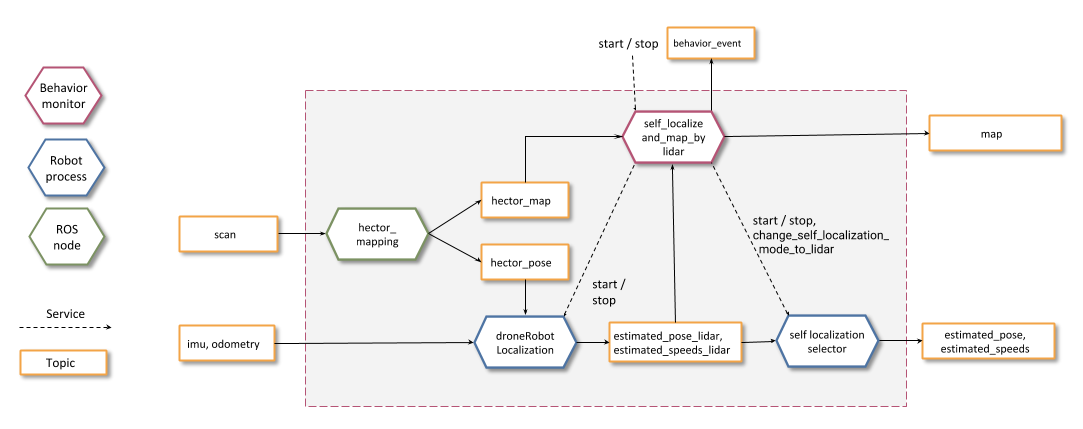
\includegraphics[width=\textwidth]{./Figures/BehaviorSlamArquitecture.png}
    \caption{Behavior self localize and map by lidar architecture. \textit{Hector mapping} is the SLAM module from \cite{hector_slam}. \textit{Drone Robot Localization} does the EKF. \textit{Self Localization Selector} gives the localization based on the selected technique.}
    \label{ch_4:fig:behav_slam}
  \end{figure}

  The estimated pose is then fed to the selector, which will toggle the localization technique. This implementation opens the door to new localization behaviors, a GPS based one for instance and also makes compatible the previous ones (visual markers based). It is easy to think of an scenario that requires both indoor and outdoor localization, in such a mission, the localization technique in use should be toggled in order for the navigator to work properly. As can be seen in Fig. \ref{ch_4:fig:behav_slam}, this is a \textit{Robot Process} with an added service to change the localization technique used.

  Bellow there is a list of the inputs and outputs of this behavior:

  % ToDo := Check this out with Martin
  [\textbf{ToDo := Set this up as a table??}]
  \begin{itemize}
  \item scan: This is the output of the lidar node, it is directly fed into the \textit{hector mapping} node
  \item imu: This topic contains the measures from the \textit{inertial measurement unit}
  \item odometry: This is a general topic with the measures from odometry
  \item map: This is the map as processed by the \textit{hector mapping} node
  \item estimated\_speed\_lidar: This is the estimated speed from the whole behavior process, fed to the selector
  \item estimated\_pose\_lidar: This is the estimated pose from the whole behavior process, fed to the selector
\end{itemize}

  This behavior monitors the correct working of the algorithm (\textit{hector mapping}) by listening on the \textit{map} topic, when it outputs strange or simply wrong data, an error is emitted.

  In the configuration file of this behavior the localization by visual markers behavior will appear as incompatible. As for the capabilities, all of \textit{hector mapping}, \textit{drone robot localization} and \textit{self localization selector} will figurate as capabilities, indicating that those processes should be started before this behavior.

\section{Navigation Interface} \label{ch_4:sect:nav_interface}

  We will consider the navigation interface as the minimum set of behaviors necessary to provide a robust, flexible API to do navigation tasks related to lidar-based localization and mapping techniques. It should be able to generate obstacle-free trajectories  to any given point (when there exists one) and be able to move the robot along those trajectories.

  The identified tasks for this API are as follows:

  \begin{enumerate}
    \item Given a point (or goal), execute the necessary motions to get the robot to that goal.
    \item Given a path, execute the necessary motions to follow it until the path is finished.
    \item Given a point (or goal), generate an obstacle-free path from the current robot's position to that goal.
  \end{enumerate}

  This tasks can be directly mapped with processes. However, we will implement them as separate behaviors to provide more modularity and reusability. Also, as each process will provide abstraction at a certain level of granularity, it makes sense to implement it as separate, independent behaviors (although some code will be duplicated)

  As of the current version of Aerostack, there exists a behavior that executes the motion of going to a given point in the 2D map representation used by Aerostack. However, this behavior is not general enough to be used with a different map representation, so we will implement a new one capable of executing the motion in the new map format: occupancy grids (which is the format used in \textit{hector mapping}). Also, in a dynamic environment, obstacles can arise in the path, this behavior will ensure that no collisions happen when executing the motion. More details to follow in section \ref{ch_4:subsect:behav_gtp}.

  The task of following a path or trajectory consists in instructing the previously available trajectory controller to follow a set of points (that conform the trajectory), given in a specific reference frame (world coordinates in this case). Contrary to the previously defined behavior, this one executes the motion blindly, providing a lower level of control to the user.

  For the last functionality, generating obstacle-free paths, another behavior will be implemented. It will consist mainly in a wrapper around the new planner, providing the lowest level of control in our navigation interface. For the planning we will employ a special planner provided as a ros package called \textit{move base}, which is specially crafted for lidar interfaces. It accepts an occupancy grid map and the raytraces from the lidar and implements the planning algorithm. Under the hood, it uses the elastic band algorithm for path optimization.

  The proposed names for each behavior are: \textit{behavior go to point in occupancy grid}, \textit{behavior follow path in occupancy grid}, \textit{behavior generate path in occupancy grid}. Figures \cref{ch_4:fig:behav_gtp,ch_4:fig:behav_fp,ch_4:fig:behav_gp} ilustrate the architecture followed by each of these behaviors. The following subsubsections explain each behavior in detail.

\subsection{Behavior Go to Point in Occupancy Grid} \label{ch_4:subsect:behav_gtp}

  This behavior provides the highest abstraction level of all the navigation interface, provided a target point, it will generate an obstacle-free trajectory to follow and send it to the trajectory controller, which executes the necessary motions to follow that trajectory. During the motion, this behavior will also ensure that no dynamic object gets in the way, recalculating the trajectory if necessary. In order to plan the trajectories, the new move base planner will be used, and as it will be a goal based behavior, the taget goal will be given as an argument to the start service. Figure \ref{ch_4:fig:behav_gtp} illustrates the general architecture of this behavior.

  \begin{figure}
    \centering
    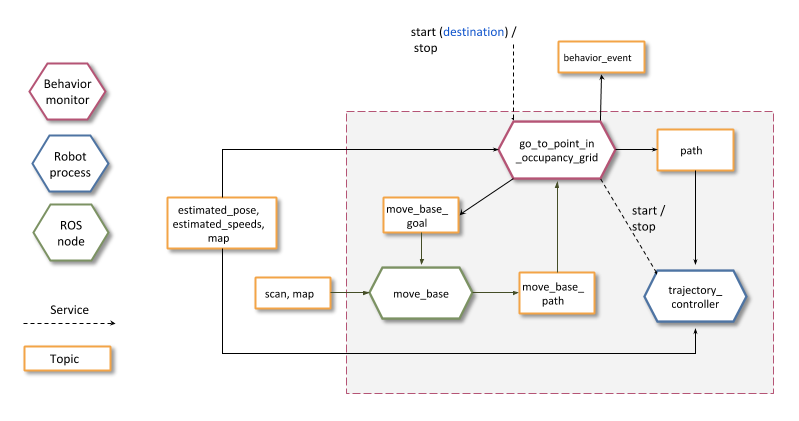
\includegraphics[width=\textwidth]{./Figures/BehaviorGTPArquitecture.png}
    \caption{Behavior Go to Point architecture. Move base is the planner}
    \label{ch_4:fig:behav_gtp}
  \end{figure}

  A condition for this behavior to operate correctly is that no other behavior is instructing the trajectory controller. To ensure this condition is met, the list of motion behaviors is stated as incompatible. The capabilities should list that it is a set-point-based flight behavior, instructing the behavior coordinator to setup the trajectory controller accordingly, the new planner (move base) should be explicitly declared as well so it is started automatically.

  \textbf{ToDo := Timeout if path not found?}

  The proposed topics will be:

  \textbf{ToDo := Set this up as a table}

  \begin{itemize}
    \item scan: Scan data from the lidar, direct input to the planner.
    \item map: Occupancy grid map from the self localize and map by lidar behavior, direct input to the planner.
    \item move base goal: Topic to instruct the planner to calculate an obstacle-free trajectory.
    \item move base path: Topic with the planned trajectory from the planner. Grabbed in the behavior to follow it.
  \end{itemize}


\subsection{Behavior Follow Path in Occupancy Grid}

  This behavior will communicate with the trajectory controller, instructing it to move following a given path received in the start service. For this behavior to work correctly, the motion behaviors should be disabled too. In this case, no other low level process is needed. The following figure illustrates the general concept (\ref{ch_4:fig:behav_fp}). Following a path can be a useful feature when developing fine grain controlled missions, like the ones enabled with Python.

  \begin{figure}[h]
    \centering
    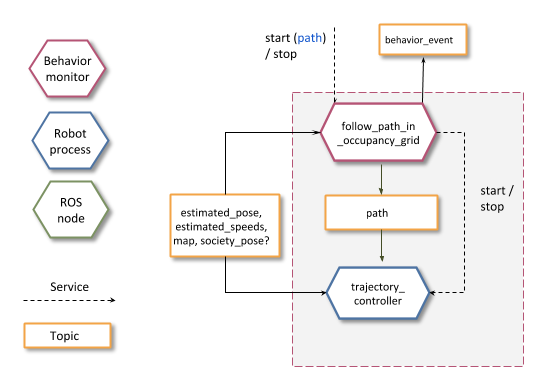
\includegraphics[width=0.75\textwidth]{./Figures/BehaviorFPArquitecture.png}
    \caption{Behavior follow path in occupancy grid architecture}
    \label{ch_4:fig:behav_fp}
  \end{figure}

  Again, the correct settings should be ensured in the configuration file, marking motion behaviors to avoid trajectories interferences.

\subsection{Behavior Generate Path in Occupancy Grid}

  In this case we will only implement a wrapper around the move base planner. This is the lowest abstraction level provided by the navigation interface API. Being able to generate paths can be useful for fine grain controlled missions and debugging. The only communication way for this behavior will be dropping the planned the path on the belief memmory, this way the amount of traffic and topics is reduced, saving computing resources and avoiding polluting more topics. It's architecture is depicted in figure \ref{ch_4:fig:behav_gp}.

  \pagebreak

  \begin{figure}[h]
    \centering
    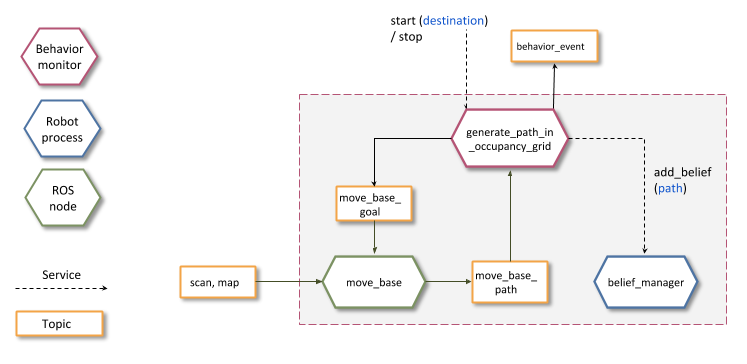
\includegraphics[width=0.85\textwidth]{./Figures/BehaviorGPArquitecture.png}
    \caption{Behavior generate path in occupancy grid architecture}
    \label{ch_4:fig:behav_gp}
  \end{figure}


This chapter has reviewed the most important aspects and specification of the implemented modules. In the next one, the validation and testing for these behaviors will be introduced.

\begin{comment}
  \begin{itemize}
  \end{itemize}
\end{comment}
 % Experimental Setup

  %\input{Chapters/Chapter4} % Experiment 1

  %\input{Chapters/Chapter5} % Experiment 2

  %\input{Chapters/Chapter6} % Results and Discussion

  %\input{Chapters/Chapter7} % Conclusion
%% ----------------------------------------------------------------
%% ----- Appendices -----------------------------------------------
  % Now begin the Appendices, including them as separate files

  \addtocontents{toc}{\vspace{2em}} % Add a gap in the Contents, for aesthetics

  \appendix % Cue to tell LaTeX that the following 'chapters' are Appendices

  \chapter{An Appendix}

Lorem ipsum dolor sit amet, consectetur adipiscing elit. Vivamus at pulvinar nisi. Phasellus hendrerit, diam placerat interdum iaculis, mauris justo cursus risus, in viverra purus eros at ligula. Ut metus justo, consequat a tristique posuere, laoreet nec nibh. Etiam et scelerisque mauris. Phasellus vel massa magna. Ut non neque id tortor pharetra bibendum vitae sit amet nisi. Duis nec quam quam, sed euismod justo. Pellentesque eu tellus vitae ante tempus malesuada. Nunc accumsan, quam in congue consequat, lectus lectus dapibus erat, id aliquet urna neque at massa. Nulla facilisi. Morbi ullamcorper eleifend posuere. Donec libero leo, faucibus nec bibendum at, mattis et urna. Proin consectetur, nunc ut imperdiet lobortis, magna neque tincidunt lectus, id iaculis nisi justo id nibh. Pellentesque vel sem in erat vulputate faucibus molestie ut lorem.

Quisque tristique urna in lorem laoreet at laoreet quam congue. Donec dolor turpis, blandit non imperdiet aliquet, blandit et felis. In lorem nisi, pretium sit amet vestibulum sed, tempus et sem. Proin non ante turpis. Nulla imperdiet fringilla convallis. Vivamus vel bibendum nisl. Pellentesque justo lectus, molestie vel luctus sed, lobortis in libero. Nulla facilisi. Aliquam erat volutpat. Suspendisse vitae nunc nunc. Sed aliquet est suscipit sapien rhoncus non adipiscing nibh consequat. Aliquam metus urna, faucibus eu vulputate non, luctus eu justo.

Donec urna leo, vulputate vitae porta eu, vehicula blandit libero. Phasellus eget massa et leo condimentum mollis. Nullam molestie, justo at pellentesque vulputate, sapien velit ornare diam, nec gravida lacus augue non diam. Integer mattis lacus id libero ultrices sit amet mollis neque molestie. Integer ut leo eget mi volutpat congue. Vivamus sodales, turpis id venenatis placerat, tellus purus adipiscing magna, eu aliquam nibh dolor id nibh. Pellentesque habitant morbi tristique senectus et netus et malesuada fames ac turpis egestas. Sed cursus convallis quam nec vehicula. Sed vulputate neque eget odio fringilla ac sodales urna feugiat.

Phasellus nisi quam, volutpat non ullamcorper eget, congue fringilla leo. Cras et erat et nibh placerat commodo id ornare est. Nulla facilisi. Aenean pulvinar scelerisque eros eget interdum. Nunc pulvinar magna ut felis varius in hendrerit dolor accumsan. Nunc pellentesque magna quis magna bibendum non laoreet erat tincidunt. Nulla facilisi.

Duis eget massa sem, gravida interdum ipsum. Nulla nunc nisl, hendrerit sit amet commodo vel, varius id tellus. Lorem ipsum dolor sit amet, consectetur adipiscing elit. Nunc ac dolor est. Suspendisse ultrices tincidunt metus eget accumsan. Nullam facilisis, justo vitae convallis sollicitudin, eros augue malesuada metus, nec sagittis diam nibh ut sapien. Duis blandit lectus vitae lorem aliquam nec euismod nisi volutpat. Vestibulum ornare dictum tortor, at faucibus justo tempor non. Nulla facilisi. Cras non massa nunc, eget euismod purus. Nunc metus ipsum, euismod a consectetur vel, hendrerit nec nunc.  % Appendix Title

  %\input{Appendices/AppendixB} % Appendix Title

  %\input{Appendices/AppendixC} % Appendix Title

  \addtocontents{toc}{\vspace{2em}}  % Add a gap in the Contents, for aesthetics
  \backmatter
%% ----------------------------------------------------------------
%% ----- Bibliography ---------------------------------------------
  \label{Bibliography}
  \lhead{\emph{Bibliography}}  % Change the left side page header to "Bibliography"
  \printbibliography
  % \bibliographystyle{unsrtnat}  % Use the "unsrtnat" BibTeX style for formatting the Bibliography
  % \bibliography{Bibliography}  % The references (bibliography) information are stored in the file named "Bibliography.bib"
%% ----------------------------------------------------------------
\end{document}  % The End
